\chapter{Facial Emotion Detection}

This section explores the facial recognition system utilised in the multimodal emotion recognition framework. It encompasses the detailed training methodologies, performance evaluations, and datasets used in the development of facial detection and emotion classification models. The section provides an in-depth analysis of the integration of various detection algorithms, including Haar cascades, dlib, and YOLO (You Only Look Once), alongside the implementation of CNN architectures MobileNetV2, VGG16, and ResNet50 for emotion detection. The comprehensive overview aims to elucidate the effectiveness and efficiency of the system in recognising and interpreting human emotions from facial expressions.

Considering the constrained computational resources inherent in robotic systems, the approach prioritises efficiency without compromising accuracy in emotion recognition. Robots often operate in resource-constrained environments, where computational overhead must be carefully managed to ensure smooth and efficient functioning. In this robot emotion recognition system, the approach is to balance accuracy and computational efficiency. Initially, the intent is to employ a Haar cascade, dlib's HOG + linear SVM, or the YOLO algorithm to locate the face within the robot's camera feed accurately. The use of these algorithms ensures that the subsequent emotion recognition model receives the expected input of only the facial region. 

\begin{figure}[!htb]
    \centering 
    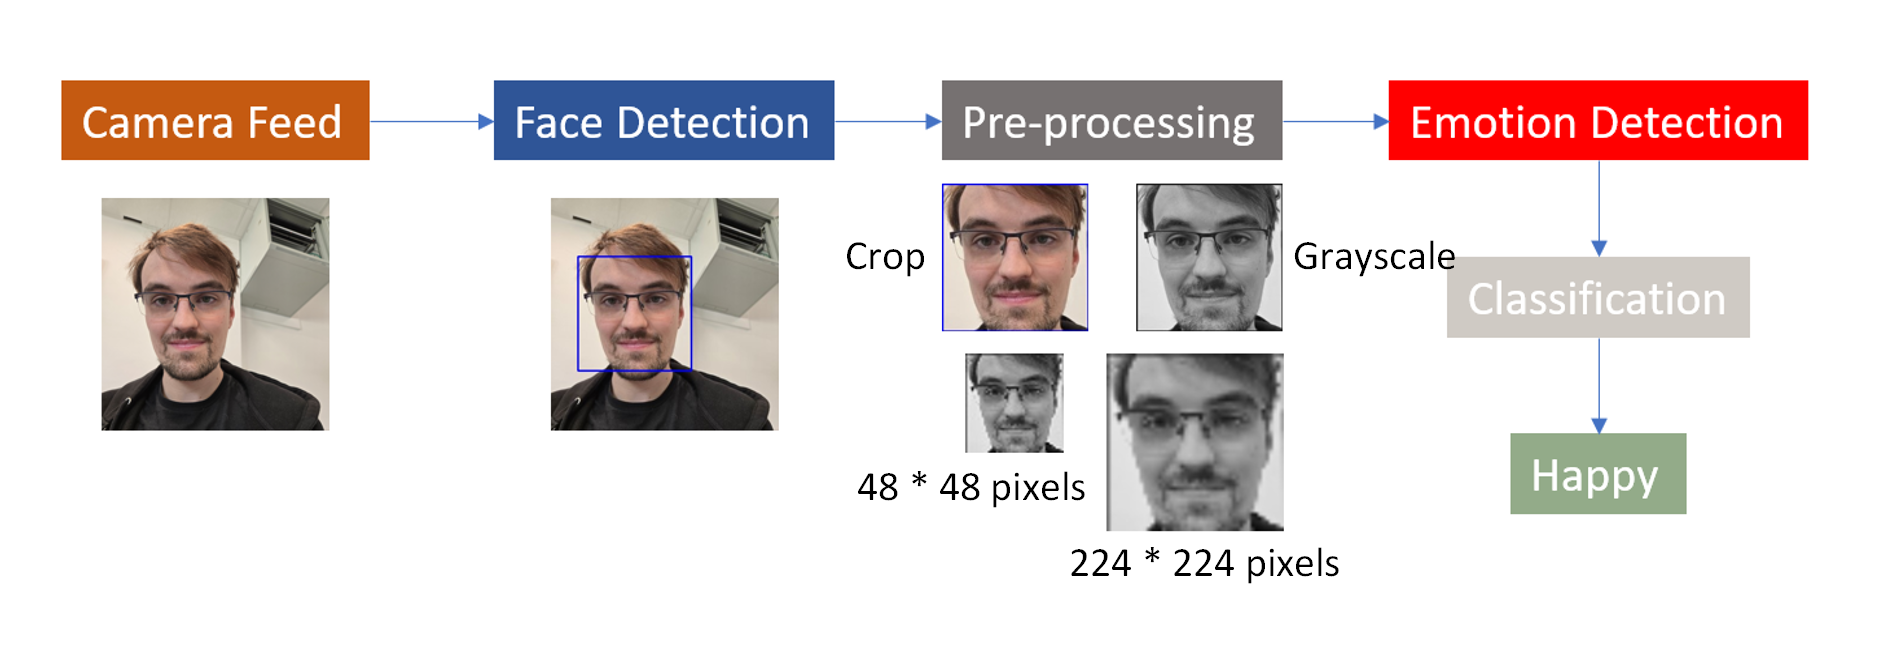
\includegraphics[scale=0.35]{fed_images/pipeline.png}
    \caption{System Pipeline}
    \label{figure:pipeline}
\end{figure}

\section{Face Detection}

\subsection{Training}

To effectively utilise YOLO, it is necessary to undergo training from scratch or fine-tuning on a specific dataset to suit the intended purpose. This entails collecting a vast dataset of labelled images where each object of interest is annotated with its bounding-box coordinates and class labels. 

The models were trained using the recommended YOLOv4 settings from the Darknet GitHub page, by changing the config file which details the training settings: batch size set to 64, subdivisions set to 16, network size width and height both set to 416, and max\_batches set to 6000. Although max\_batches is typically calculated as the number of classes multiplied by 2000, which would result in 2000 for a single class, the minimum allowable value is 6000. Therefore, this value was adjusted accordingly to meet the training requirements.

Then the layers are slightly altered to match the number of classes. Each [yolo] layer has a classes section, this results in changing 3 total layers to have 1 instead of the default 80. Finally, just before each [yolo] layer is a [convolutional] layer that needs the filter settings lowering from the default 255 to (classes + 5) * 3, thus these are set to 18. Changing this setting allows the model to predict only one class.

Changing the Tiny-YOLO config follows the same process as full YOLO; however, there are only 2 [yolo] layers instead of 3. Lastly, both models have their own pre-trained weights file that was included to assist with training. The final command used in each is shown below.

\noindent See the following commands:
\begin{lstlisting}[language=bash]
  $ ./darknet detector train data/obj.data \
        yolov4_face.cfg data/yolov4.conv.137 -map -gpus 0,1
  $ ./darknet detector train data/obj.data \
        yolov4_tiny_face.cfg data/yolov4-tiny.conv.29 \
            -map -gpus 0,1
\end{lstlisting}


\subsection{Dataset}

Both models are trained on the WIDER FACE \cite{yang2016wider} dataset, a well-known dataset for face recognition and detection tasks. This data set consists of a large number of images annotated with faces at various scales, positions, and levels of occlusion, making it a challenging and diverse data set that is ideal for testing object detection models.

The WIDER FACE dataset has been meticulously crafted to support face detection and recognition algorithms research. It has 12,878 images in the training set and 3,224 images in the validation set sourced from different locations, featuring an extensive assortment of scenes, lighting conditions, poses, and occlusions. This data set is uniquely annotated with precise boundary boxes around each face in every image, providing a reliable basis for training and evaluation purposes.

Each image in this dataset has been annotated with one or more bounding boxes, which capture information about each face's position, orientation, and scale. These annotations effectively encompass the diversity of face sizes and poses in different images, including occluded faces. This data set is exceptional in its capacity to evaluate the robustness of face detection algorithms under challenging conditions.

The WIDER FACE dataset is distinguished by its rich diversity in subjects, scenes, and environmental conditions. It contains images captured in different settings, such as indoor and outdoor scenes, crowded environments, street scenes, and surveillance footage. It features faces of numerous genders, ages, ethnicities, and facial expressions, ensuring a comprehensive representation of real-world scenarios.

An evaluation of YOLO and Tiny YOLO’s performance will be done on both the complete dataset and a couple chosen subsets. One subset comprises images containing only one face per image, providing a more focused and simplified training scenario. This approach allows for targeted experimentation and analysis, enabling insights into the model's performance and robustness in scenarios with minimal occlusions or distractions from multiple faces. The resulting size of this dataset is 1,342 images in the training set and 334 images in the validation set. The other subset contains all the images that featured more than one face; this should reveal if the models have any issues with higher complexity images. This set has 8245 in the training set and 2104 images in the validation set.

\subsection{Performance}

To ensure the effectiveness of the YOLO model in detecting faces for subsequent emotion recognition tasks, its performance is evaluated using a variety of metrics. These metrics offer a comprehensive view of the accuracy, speed, and robustness of the model.

In this section, the performance of the YOLO and Tiny YOLO object detection models was evaluated on a face detection dataset: the Wider Face dataset. This dataset was then split into images containing multiple faces, and images containing only one face. The metrics used for the evaluation include precision, recall, F1 score, average Intersection over Union (IoU), and Average Precision (AP).

Precision measures the accuracy of positive predictions. It is calculated as the ratio of true positives (correctly detected faces) to the sum of true positives and false positives (incorrect detections). High precision means that most of the faces detected by the model are actual faces.

\[
\text{Precision} = \frac{\text{True Positives}}{\text{True Positives} + \text{False Positives}}
\]
 
Recall, or sensitivity, measures the ability of the model to find all relevant instances. It is the ratio of true positives to the sum of true positives and false negatives (missed detections). High recall means that the model can detect most if not all of the faces present in a given image.

\[
\text{Recall} = \frac{\text{True Positives}}{\text{True Positives} + \text{False Negatives}}
\]

The F1 score is the harmonic mean of precision and recall, providing a single metric to evaluate the model's overall performance. It balances the trade-off between precision and recall and is especially useful as an evaluation metric in binary classification.

\[
\text{F1} = 2 \times \frac{\text{Precision} \times \text{Recall}}{\text{Precision} + \text{Recall}}
\]

Intersection over Union measures the overlap between the predicted bounding box and the ground truth bounding box. It is calculated by dividing the overlap area by the union area between the two boxes. A higher IoU means the predicted bounding box closely matches the actual bounding box.

\[
\text{IoU} = \frac{\text{Area of Overlap}}{\text{Area of Union}}
\]
 
Average Precision is a weighted mean of precision scores, where the weight is the increase in recall from the previous threshold. A high AP means that a model has a low false negative and false positive rate.

\begin{table}[h!]
\centering
\caption{Performance of YOLO on Full Wider Face and Single Face Datasets}
\begin{tabular}{|l|c|c|c|}
\hline
\textbf{Metric}      & \textbf{Full Wider Face} & \textbf{Multi Face}  & \textbf{Single Face} \\ \hline
\textbf{Precision}   & 0.61        & 0.61            & 0.95                 \\ \hline
\textbf{Recall}      & 0.64        & 0.63            & 0.92                 \\ \hline
\textbf{F1 Score}    & 0.63        & 0.62            & 0.94                 \\ \hline
\textbf{Average IoU} & 45.77\%     & 45.12\%            & 80.90\%              \\ \hline
\textbf{AP}          & 63.17\%     & 62.11\%              & 97.39\%              \\ \hline
\end{tabular}
\label{tab:YOLO}
\end{table}

\begin{table}[h!]
\centering
\caption{Performance of Tiny YOLO on Full Wider Face and Single Face Datasets}
\begin{tabular}{|l|c|c|c|}
\hline
\textbf{Metric}      & \textbf{Full Wider Face} & \textbf{Multi Face}  & \textbf{Single Face} \\ \hline
\textbf{Precision}   & 0.48        & 0.47            & 0.95                 \\ \hline
\textbf{Recall}      & 0.44        & 0.43            & 0.91                 \\ \hline
\textbf{F1 Score}    & 0.46        & 0.45            & 0.93                 \\ \hline
\textbf{Average IoU} & 35.32\%     & 34.46\%            & 78.08\%              \\ \hline
\textbf{AP}          & 36.63\%     & 35.04\%             & 92.33\%              \\ \hline
\end{tabular}

\label{tab:TINYYOLO}
\end{table}

Tables \ref{tab:YOLO} and \ref{tab:TINYYOLO} summarise the performance of the YOLO and Tiny YOLO models, respectively, on the 3 datasets.

The results in the tables show an interesting development. Whilst the full YOLO model performs markedly better when there are multiple faces in the image compared to its Tiny counterpart, when it comes to detections where only a single face is present in the image, there is no discernible difference between the two except a slight reduction in the average IoU and average precision. The results on the version of the dataset with only multiple faces backs up the hypothesis that Tiny YOLO struggles with the higher complexity images. Thus, in this system's intended use case (a human-robot 1-on-1), Tiny YOLO is more than sufficient to perform face detection.

In addition to YOLO and Tiny YOLO, the performance of Haar Cascade and dlib’s HOG+Linear SVM was evaluated on the same datasets. However since these two models do not provide confidence scores along with their predictions, the metric AP cannot be calculated. AP is derived from the precision-recall curve, where predictions are ranked by their confidence scores. The curve is created by varying a confidence threshold, recalculating precision and recall at different confidence levels. Without confidence scores, every prediction is treated equally, leading to an uninformative or flat curve, which won't reflect the model's ability to prioritise better predictions.

\begin{table}[h!]
\centering
\caption{Performance of Haar Cascade on Full Wider Face and Single Face Datasets}
\begin{tabular}{|l|c|c|c|}
\hline
\textbf{Metric}      & \textbf{Full Wider Face} & \textbf{Multi Face}  & \textbf{Single Face} \\ \hline
\textbf{Precision}   & 0.69      &  0.74           & 0.45               \\ \hline
\textbf{Recall}      & 0.15      &  0.14           & 0.69               \\ \hline
\textbf{F1 Score}    & 0.25      &  0.24           & 0.55               \\ \hline
\textbf{Average IoU} & 69.64\%     &  69.63\%           & 69.36\%              \\ \hline
\end{tabular}
\label{tab:HAAR}
\end{table}

\begin{table}[h!]
\centering
\caption{Performance of HOG+Linear SVM on Full Wider Face and Single Face Datasets}
\begin{tabular}{|l|c|c|c|}
\hline
\textbf{Metric}      & \textbf{Full Wider Face} & \textbf{Multi Face}  & \textbf{Single Face} \\ \hline
\textbf{Precision}   & 0.96       & 0.97           & 0.94               \\ \hline
\textbf{Recall}      & 0.14       & 0.12           & 0.78               \\ \hline
\textbf{F1 Score}    & 0.24       & 0.22           & 0.86               \\ \hline
\textbf{Average IoU} & 69.61\%      & 69.91\%           & 66.35\%              \\ \hline
\end{tabular}
\label{tab:HOGSVM}
\end{table}

Tables \ref{tab:HAAR} and \ref{tab:HOGSVM} present the performance of the Haar Cascade and HOG + Linear SVM models, respectively, on the full Wider Face dataset and a single face dataset.

These results indicate that both the Haar Cascade and HOG+Linear SVM models, unlike YOLO and Tiny YOLO, perform better on the more complex detection task of the Full Wider face dataset. The high precision but low recall of both models on the full Wider Face dataset and the multiple face subset suggests that they are more conservative in detections, leading to fewer false positives but more false negatives. These initial tests were conducted on the high-powered training machine, clearly highlighting the difference in model complexity by the time taken to complete the tests on the validation sets, the Haar Cascade took a total of 295.36 seconds. In comparison, the HOG+Linear SVM took 1402.19 seconds.

\section{Emotion Detection}
\subsection{Datasets}
\subsubsection{Training}

The datasets selected for emotion detection training were FERPlus \cite{BarsoumICMI2016} and an altered version of CK+ \cite{5543262}. Both datasets are downloaded from publicly available databases online. FERPlus and CK+ both contain images of unconstrained facial expressions. A sample of images from FERPlus and CK+ are shown in figure \ref{figure:sample_imgs}. 

\begin{figure}[!htb]
    \centering 
    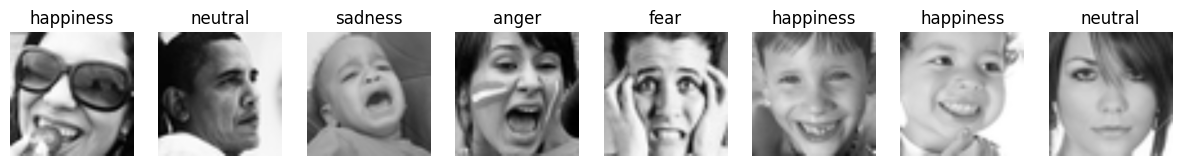
\includegraphics[scale=0.5]{fed_images/random_imgs.png}
    \caption{Sample of images from the combined dataset of FER+ and CK+}
    \label{figure:sample_imgs}
\end{figure}

The FERPlus database is a derivative of the original FER2013 dataset. FER2013 suffered from several issues that made the dataset difficult to perform recognition tasks on, these issues include non-face data and false labels resulting in even state-of-the-art models reaching around 60\%-70\% accuracy. FERPlus results from 10 crowd-sourced taggers relabelling the original dataset to provide better quality ground truth for still image emotion than the original FER labels. The taggers categorised each image into one of 10 different labels: 8 emotions (happiness, neutral, sadness, surprise, fear, disgust, contempt, and anger) and 2 additional categories representing cases where the emotion is indeterminate or the image does not contain a human face (unknown and non-face). To remove uncertain images and filter each image into a single labelled folder, a maximum voting method was implemented. This results in 28,386 samples in the training set, 3546 in the private test set and 3,553 in the public test set. \ref{tab:emotion_distribution} indicates the number of images in each emotion category.

\begin{table}[h!]
\centering
\caption{Emotion distribution of the training dataset}
\begin{tabular}{|l|c|c|c|c|}
\hline
\textbf{Emotion}   & \textbf{PrivateTest} & \textbf{PublicTest} & \textbf{Training} & \textbf{Total} \\ \hline
\textbf{Anger}     & 325                  & 319                 & 2,466             & 3,110          \\ \hline
\textbf{Contempt}  & 27                   & 24                  & 165               & 216            \\ \hline
\textbf{Disgust}   & 23                   & 34                  & 191               & 248            \\ \hline
\textbf{Fear}      & 93                   & 74                  & 652               & 819            \\ \hline
\textbf{Happiness} & 928                  & 899                 & 7,528             & 9,355          \\ \hline
\textbf{Neutral}   & 1,262                & 1,335               & 10,308            & 12,905         \\ \hline
\textbf{Sadness}   & 444                  & 412                 & 3,514             & 4,370          \\ \hline
\textbf{Surprise}  & 444                  & 456                 & 3,562             & 4,462          \\ \hline
\textbf{Total}     & 3,546                & 3,553               & 28,386            & 35,485         \\ \hline
\end{tabular}
\label{tab:emotion_distribution}
\end{table}

The dataset is heavily skewed towards the 'Happiness' (9,355 images) and 'Neutral' (12,905 images) categories. These categories collectively represent over 62\% of the entire dataset. Such a high representation can result in a bias or overfitting \cite{Rangulov2020-pd} towards these emotions, reducing its sensitivity and accuracy in detecting less represented emotions.

However, emotions such as 'Contempt' (216 images), 'Disgust' (248 images), and 'Fear' (819 images) are significantly under-represented. The model might not learn to recognise these emotions effectively due to the limited examples available, leading to poor performance in real-world scenarios where these emotions are present. Emotions like 'Anger' (3,110 images), 'Sadness' (4,370 images), and 'Surprise' (4,462 images) have a moderate number of samples but still far less compared to 'Happiness' and 'Neutral'. Although better than the least represented categories, the imbalance still poses a risk of the model underperforming in these emotions.

CK+ or Extended Cohn-Kanade dataset consists of 593 video sequences from 123 subjects ranging from 18 to 50 years old. Gender and heritage of participants varied with 69\% female, 81\%, Euro-American, 13\% Afro-American, and 6\% other groups. Each video shows a facial shift from a neutral expression to a targeted peak expression, recorded at 30 frames per second (FPS) at a resolution of 640x480 pixels. These videos are labelled into one of seven emotions: anger, contempt, disgust, fear, happiness, sadness, and surprise. This data needs to be in a format similar to the FERPlus dataset, 48x48 in greyscale. On a database-sharing website, Kaggle, there is a version of CK+ in this format, below is the information provided alongside the database: 

\begin{itemize}
    \item Contains adapted data up to 920 images from 920 original CK+ dataset
    \item Data is already reshaped to 48x48 pixels, in grayscale format and facecropped using haarcascade\_frontalface\_default.
    \item Noisy (based on room light/hair format/skin colour) images were adapted to be clearly identified using Haar classifier.
    \item Columns from file are defined as emotion/pixels/Usage
\end{itemize}

The resulting number of images in each emotion category is detailed in \ref{tab:emotion_counts_ck+}.

\begin{table}[h!]
\centering
\caption{Image counts for each emotion in CK+}
\begin{tabular}{|l|c|}
\hline
\textbf{Emotion}   & \textbf{Count} \\ \hline
\textbf{Anger}     & 135   \\ \hline
\textbf{Contempt}  & 54    \\ \hline
\textbf{Disgust}   & 177   \\ \hline
\textbf{Fear}      & 75    \\ \hline
\textbf{Happiness} & 207   \\ \hline
\textbf{Sadness}   & 84    \\ \hline
\textbf{Surprise}  & 249   \\ \hline
\end{tabular}
\label{tab:emotion_counts_ck+}
\end{table}

\subsubsection{Preprocessing}

To ensure compatibility and consistency across VGG16, ResNet50, and MobileNetV2 models, the FER and CK+ datasets undergo specific preprocessing steps.

Firstly, all images are resized from 48x48 to 224x224 pixels. This resizing is necessary because, while VGG16 and MobileNetV2 can be adjusted to accept 48x48 images, ResNet50 could not process the images at 48x48 and required a minimum size of 224x224. Resizing all images to 224x224 ensures uniformity across all models.

Secondly, the images, originally in greyscale, need to be converted to have three channels as required by the models. This is achieved using OpenCV to convert single-channel greyscale images to three-channel images using cv2.cvtColor() with the constant cv2.COLOR\_GRAY2BGR. 

Lastly, normalisation is specifically required for VGG16. The images are reshaped for normalisation using the StandardScaler from the sklearn.preprocessing Python library and then reshaped back to its original dimensions. This normalisation step ensures that the input data is standardised, which is crucial for the performance of VGG16.

In addition to these pre-processing steps, data augmentation techniques are applied to enhance the robustness of the models, prevent overfitting, and alleviate the issue of the unbalanced data set. Data augmentation involves artificially increasing the size of the training dataset by generating new training samples from the original data. This can be done through geometric transformations such as width and height shifts, horizontal flips, and zooming as well as many other techniques such as GAN (General Adversarial Networks) and Photometric Transformations \cite{Shorten2019-mj}. These transformations help the models generalise better by exposing them to various image conditions and distortions they might encounter in real-world scenarios.

Specifically, the following augmentations are applied:

\begin{itemize}
\item Width and Height Shifts: Images are randomly shifted horizontally and vertically by up to 10\% of the image width and height (width\_shift\_range = 0.1 and height\_shift\_range = 0.1).
\item Horizontal Flip: Images are randomly flipped horizontally to simulate different viewing angles (horizontal\_flip = True).
\item Zoom: Random zooms in and out within a range of 0.8 to 1.2 times the original size are applied (zoom\_range = 0.2).
\end{itemize}

These augmentations are performed using the ImageDataGenerator class from the Keras library, which allows for real-time data augmentation during the training process. By applying these augmentations, the diversity of the training data is significantly increased.

\subsection{Training}

After processing the base convolutional layers of each pretrained model (VGG16, ResNet50, and MobileNetV2), the feature maps were flattened using the flatten() function.

The output layer of each model was configured to match the number of emotion classes in the dataset. This layer used a dense layer with the number of neurones equal to the number of classes and a softmax activation function to provide a probability distribution as the resulting prediction.

The models were then trained using the Adam optimiser with an initial learning rate of 0.001 and a batch size of 64. The models were trained for 50 epochs. The categorical cross-entropy loss function was used to optimise the model.

\begin{figure}[H]
    \centering 
    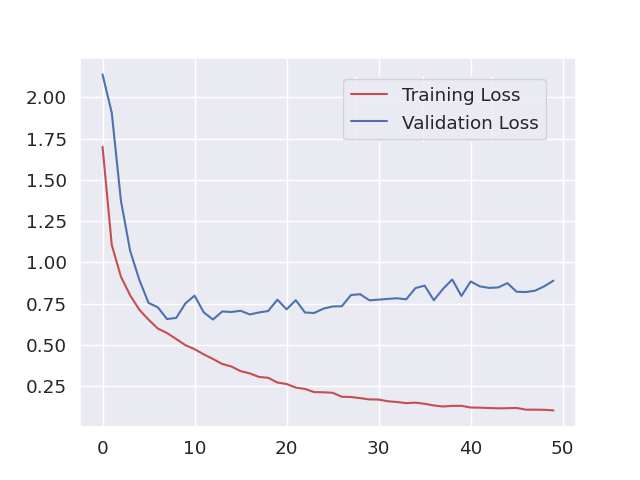
\includegraphics[scale=0.5]{fed_images/train_loss_MobileNetv2.png}
    \caption{The loss graph for the first successful training of MobileNetV2}
    \label{figure:loss_mnv2}
\end{figure}

The graph \ref{figure:loss_mnv2} illustrates the training and validation loss for the MobileNetV2 model. As training progresses, both losses decrease sharply, demonstrating that the model is learning from the data. Around the 20-epoch mark, the training loss continues to decline steadily, indicating that the model is fitting well to the training data. The validation loss begins to see a slight upward trend after around 11 epochs suggesting that the model is overfitting as the training loss continues to decrease.

\begin{figure}[H]
    \centering 
    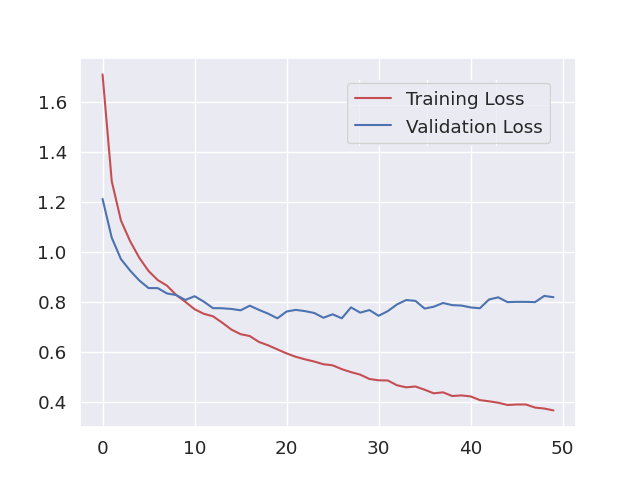
\includegraphics[scale=0.5]{fed_images/train_loss_ResNet50.png}
    \caption{The loss graph for the first successful training of ResNet50}
    \label{figure:loss_rn50}
\end{figure}

Graph \ref{figure:loss_rn50} shows the training and validation loss for the ResNet50 model. Similar to MobileNetV2, both losses start high and decrease significantly in the early epochs. The training loss for ResNet50 drops more quickly and smoothly compared to the validation loss, reaching a much lower value as epochs progress. The validation loss shows a decreasing trend but with more pronounced fluctuations, indicating some instability in performance on the validation set. After around 30 epochs the validation loss starts a slight upward trend. By the end of the 50 epochs, the training loss is significantly lower than the validation loss, which might suggest slight overfitting.

\begin{figure}[H]
    \centering 
    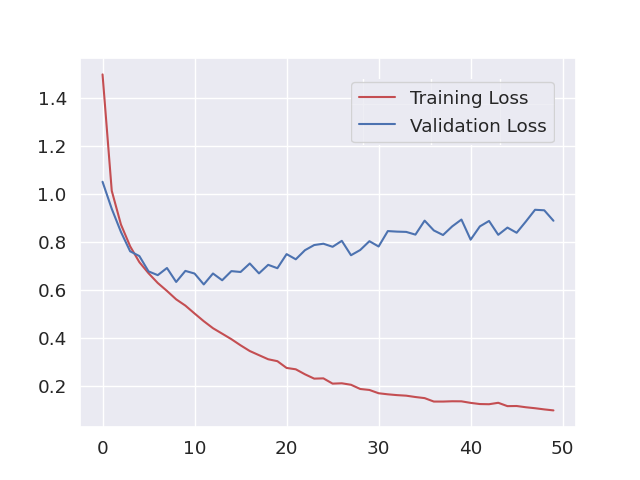
\includegraphics[scale=0.5]{fed_images/train_loss_VGG16.png}
    \caption{The loss graph for the first successful training of VGG16}
    \label{figure:loss_vgg16}
\end{figure}

Finally, graph \ref{figure:loss_vgg16} represents the training and validation loss for the VGG16 model. Both losses start high and decrease rapidly in the initial epochs, similarly to the other models. However, the training loss for VGG16 continues to decrease more steeply and steadily, reaching very low values, indicating a strong fitting to the training data. The validation loss decreases initially but starts to exhibit more fluctuation and even an upward trend after around 11 epochs. This divergence between training and validation loss suggests that VGG16 might be overfitting to the training data, capturing noise and details that do not generalise well to the validation set.

To further mitigate the impact of overfitting in the three emotion recognition models a few more techniques were added. Firstly an early stopper was added, this, with a patience set at 10, stops the training of the model if no improvements are made after 10 epochs of training and a checkpointer that will restore the model to the best weights. Alongside this, a reduced learning rate was implemented that lowers the learning rate if the training starts to hit a plateau in accuracy. 

\begin{figure}[H]
    \centering 
    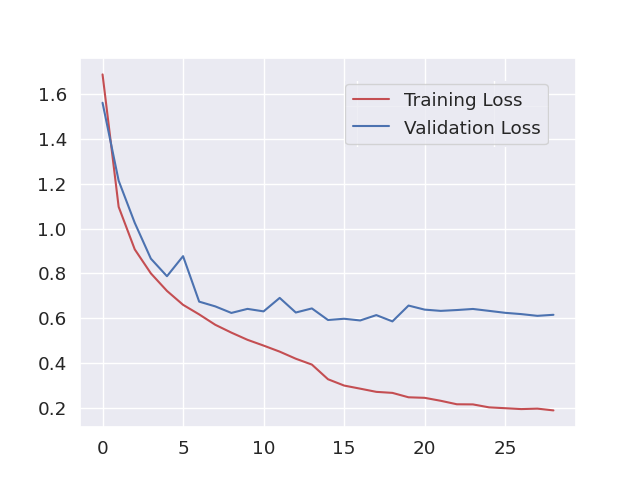
\includegraphics[scale=0.5]{fed_images/train_loss_MobileNetv2_ofp.png}
    \caption{The loss graph for the second successful training of MobileNetV2}
    \label{figure:loss_mnv2_ofp}
\end{figure}

MobileNetV2s second training loss graph is shown in figure \ref{figure:loss_mnv2_ofp}. The graph shows that the training only got to 29 epochs before the early stopper function stopped it. The application of techniques to prevent overfitting seems effective. The gap between training and validation loss is relatively small. The model continues to improve on both training and validation data, indicating that it is learning useful patterns rather than just memorising the training data. The stabilisation of the validation loss suggests that the model has reached a point where further training may yield diminishing returns.

\begin{figure}[H]
    \centering 
    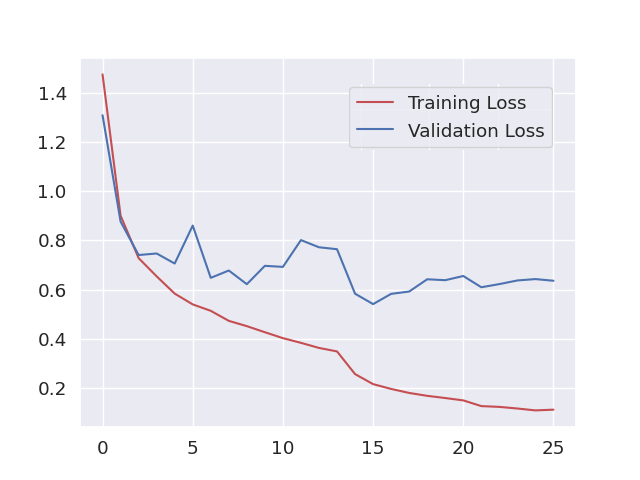
\includegraphics[scale=0.5]{fed_images/train_loss_ResNet50_ofp.png}
    \caption{The loss graph for the second successful training of ResNet50}
    \label{figure:loss_rn50_ofp}
\end{figure}

ResNet50’s second training results in a similar graph to its first run. After only 5 epochs validation loss begins to fluctuate increasing and decreasing until around epochs 15 to 25, where the validation loss shows a slight upward trend.

\begin{figure}[H]
    \centering 
    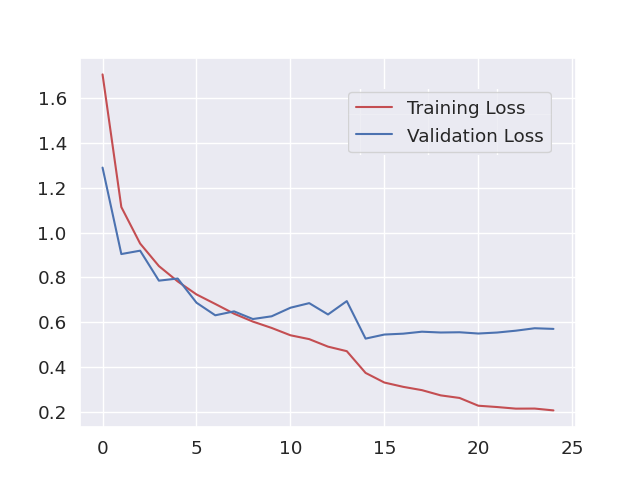
\includegraphics[scale=0.5]{fed_images/train_loss_VGG16_ofp.png}
    \caption{The loss graph for the second successful training of VGG16}
    \label{figure:loss_vgg16_ofp}
\end{figure}

In the second training run of VGG16 after about 5 epochs, the validation loss begins to fluctuate, while the training loss continues to decrease steadily. From Epochs 10 to 25, the validation loss shows a slight downward trend with occasional fluctuations, indicating potential minor overfitting. However, the training loss continues to decrease smoothly, suggesting that the model is still learning effectively. Overall, the model demonstrates good generalisation, and the techniques applied seem to mitigate the severe overfitting it saw in the first run.

\begin{figure}[H]
    \centering 
    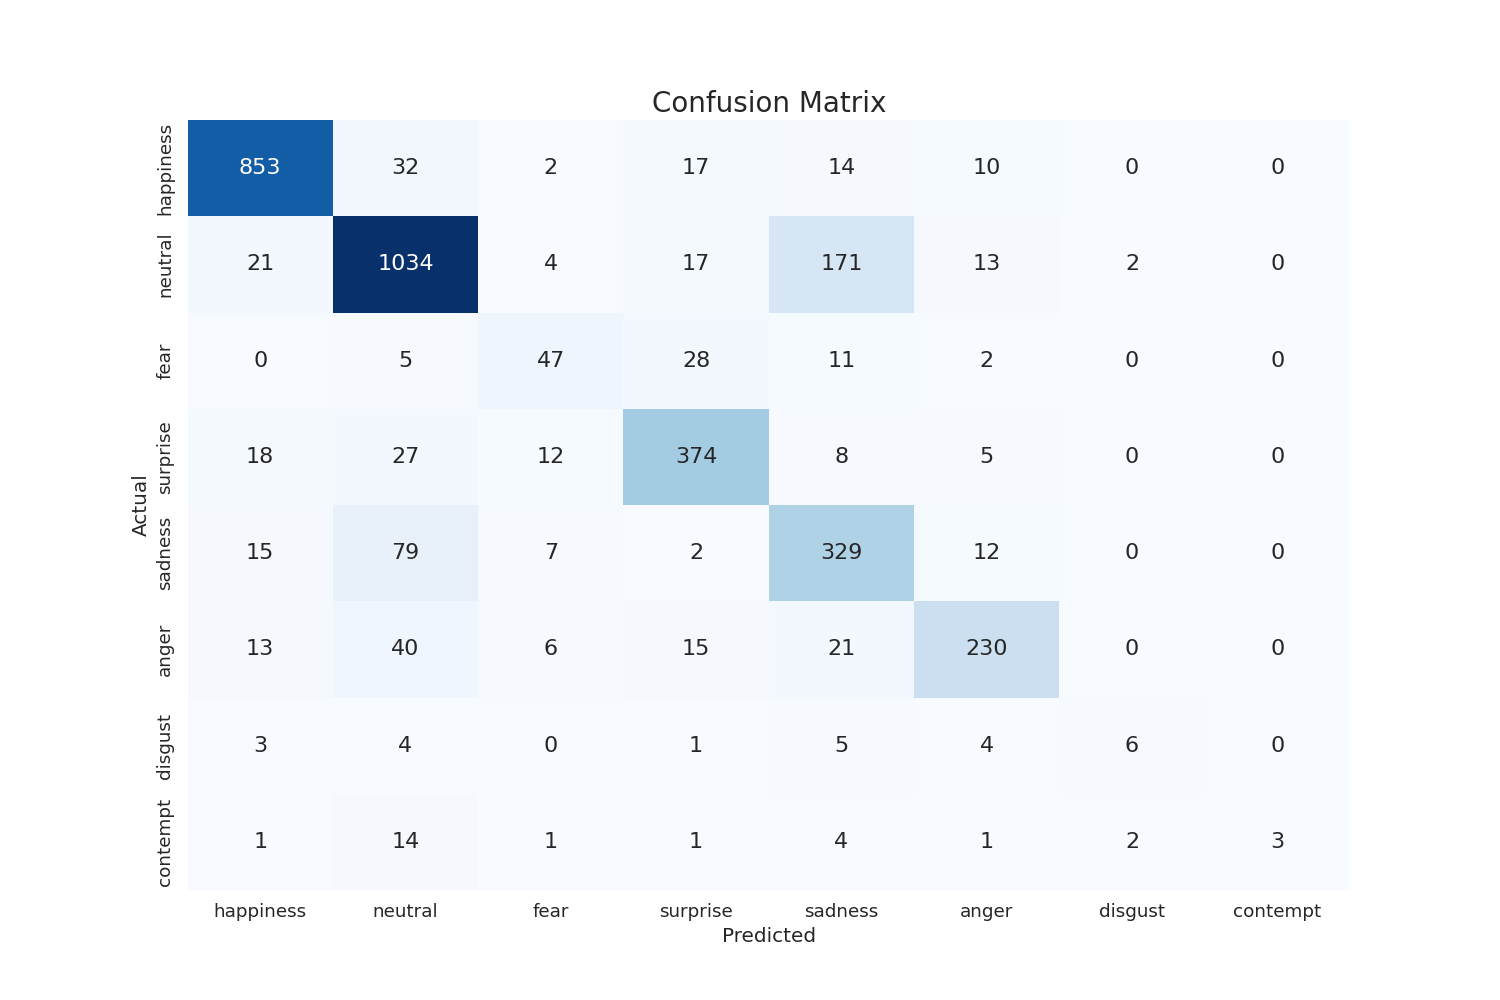
\includegraphics[scale=0.38]{fed_images/conf_matrix_MobileNetv2.png}
    \caption{The confusion matrix detailing the performance of MobileNetV2 on the PrivateTest set}
    \label{figure:conf_mnv2}
\end{figure}

The confusion matrix \ref{figure:conf_mnv2} illustrates the performance of MobileNetV2 across the 8 emotions. The model accurately classifies the 'happiness' and 'neutral' expressions, with 853 and 1034 correct predictions, respectively. However, it struggles with 'fear' and 'contempt', frequently misclassifying them as other emotions. There is notable confusion between 'sadness' and 'neutral' with it incorrectly classifying them as each other. 

Figure \ref{figure:sadneutral} shows an example of images from sadness and neutral. The confusion could be attributed to the subtle facial differences between 'sadness' and 'neutral' expressions. Both emotions tend to exhibit minimal facial muscle movement, and the lack of exaggerated features such as smiles or frowns can make it challenging for models to distinguish between them.

\begin{figure}[H]
    \centering 
    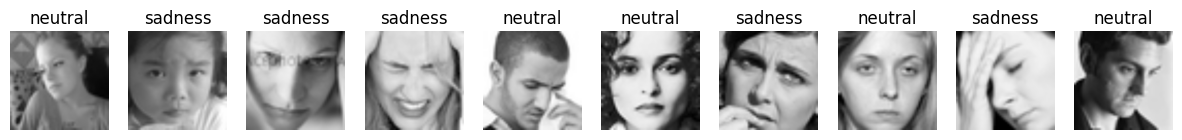
\includegraphics[scale=0.38]{fed_images/sadness+neutral.png}
    \caption{Example images showing the very slight variation between sadness and neutral}
    \label{figure:sadneutral}
\end{figure}

\begin{figure}[H]
    \centering 
    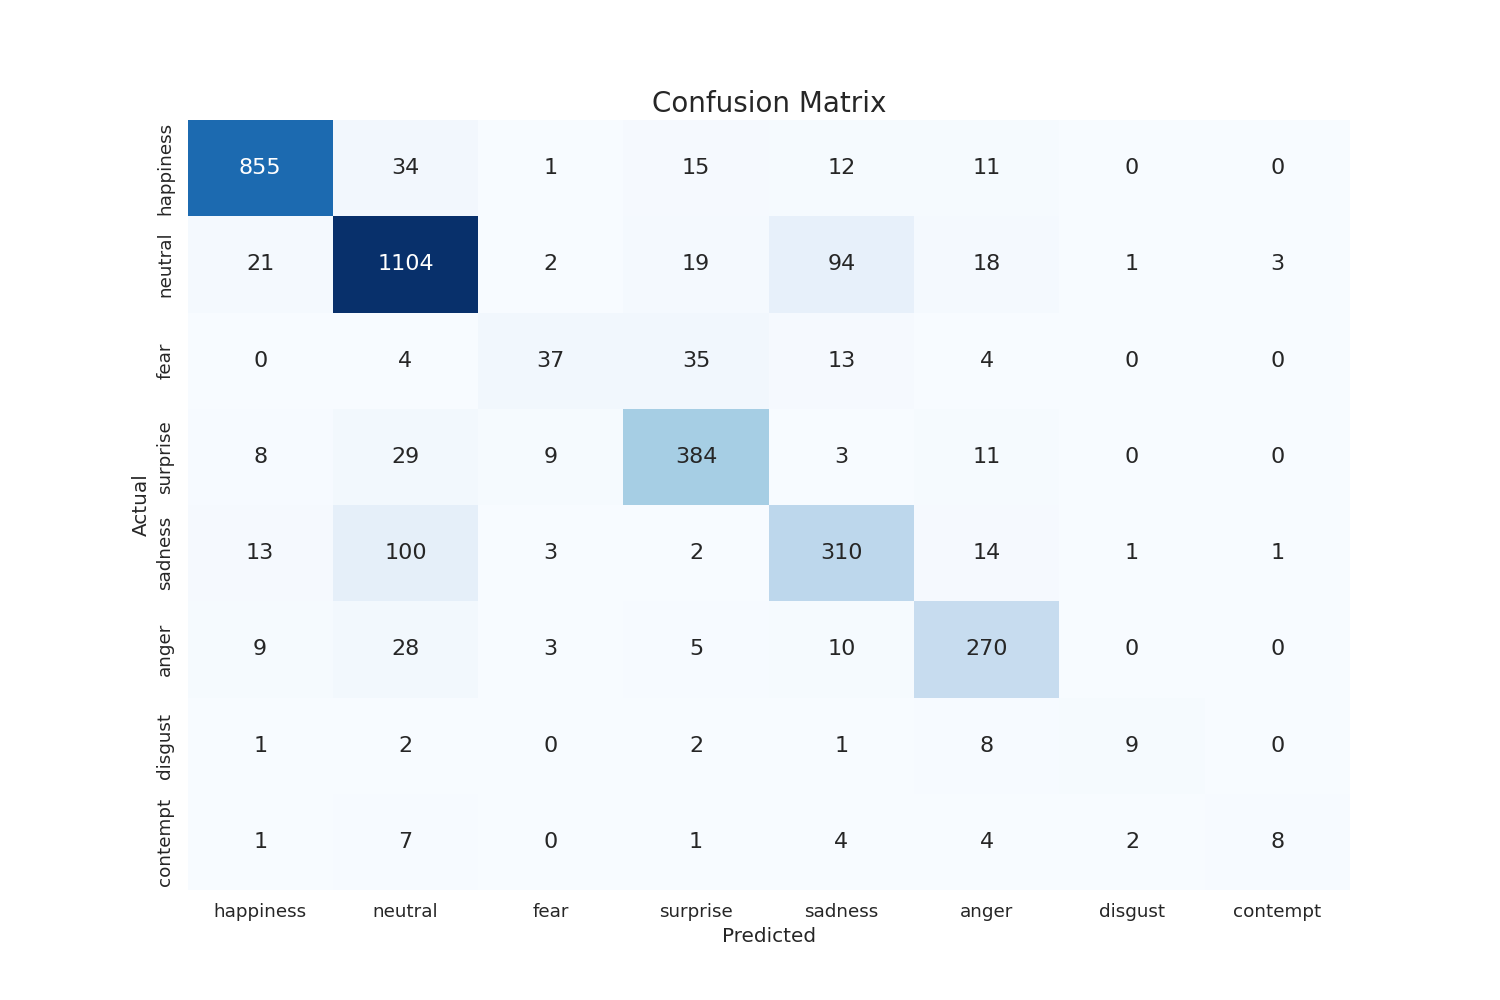
\includegraphics[scale=0.38]{fed_images/conf_matrix_ResNet50.png}
    \caption{The confusion matrix detailing the performance of ResNet50 on the PrivateTest set}
    \label{figure:conf_rn50}
\end{figure}

ResNet50 performed very similarly to MobileNetV2 but had a slightly higher recognition rate for each emotion except ‘fear’ and ‘sadness’. It suffers from the same misclassification of ‘sadness’ and ‘neutral’ as MobileNetV2. 

\begin{figure}[H]
    \centering 
    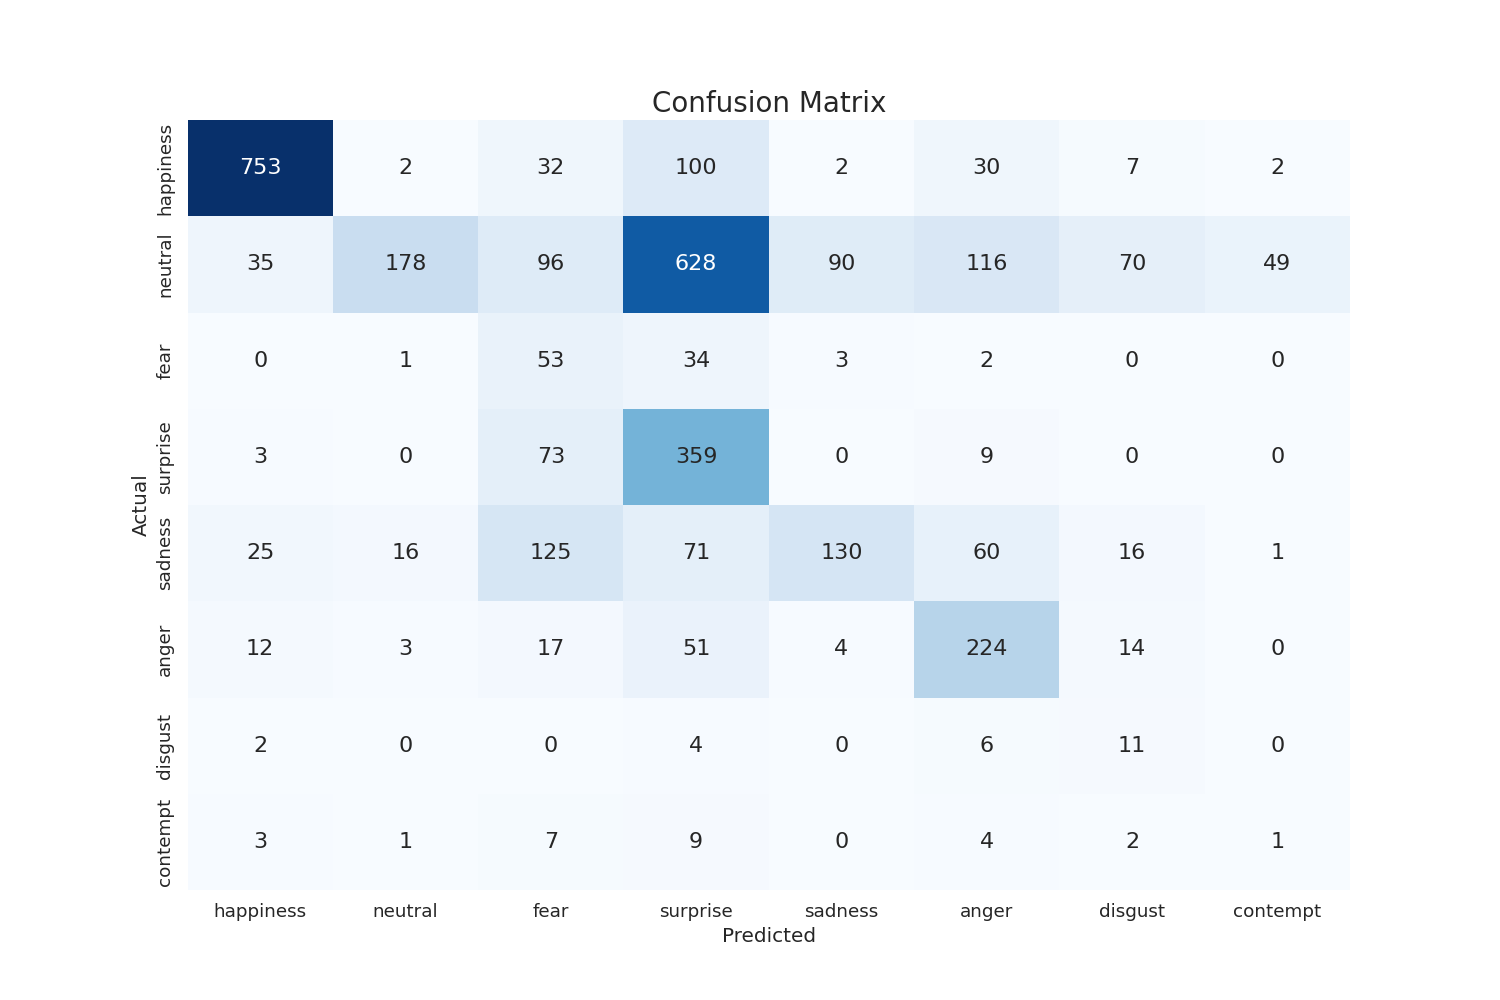
\includegraphics[scale=0.38]{fed_images/conf_matrix_VGG16.png}
    \caption{The confusion matrix detailing the performance of VGG16 on the PrivateTest set}
    \label{figure:conf_vgg16}
\end{figure}

VGG16 misclassified most of the 'neutral' pictures, only getting 178 correct, mainly classifying them as ‘surprise’ and ‘anger’. However, VGG16 achieved the highest results of the three models in the fear category. The model also struggles to differentiate between ‘sadness’ and ‘fear’. Overall, the model does perform well; however, in comparison to ResNet50 and MobileNetV2, it misclassifies too many emotions to be considered reliable.

\subsection{Testing}

This section evaluates the performance of three emotion recognition models in conjunction with face detection algorithms: Haar cascades, dlib, Tiny YOLO and YOLO. The evaluation is conducted using the Expression in-the-Wild (ExpW) dataset, which contains facial images captured in diverse and unconstrained environments. This comprehensive testing aims to assess the robustness and accuracy of the models and algorithms in recognising emotions under varied and challenging scenarios.

A selection of random images from ExpW can be seen in \ref{figure:exp_w_sample}.

\begin{figure}[!htb]
    \centering 
    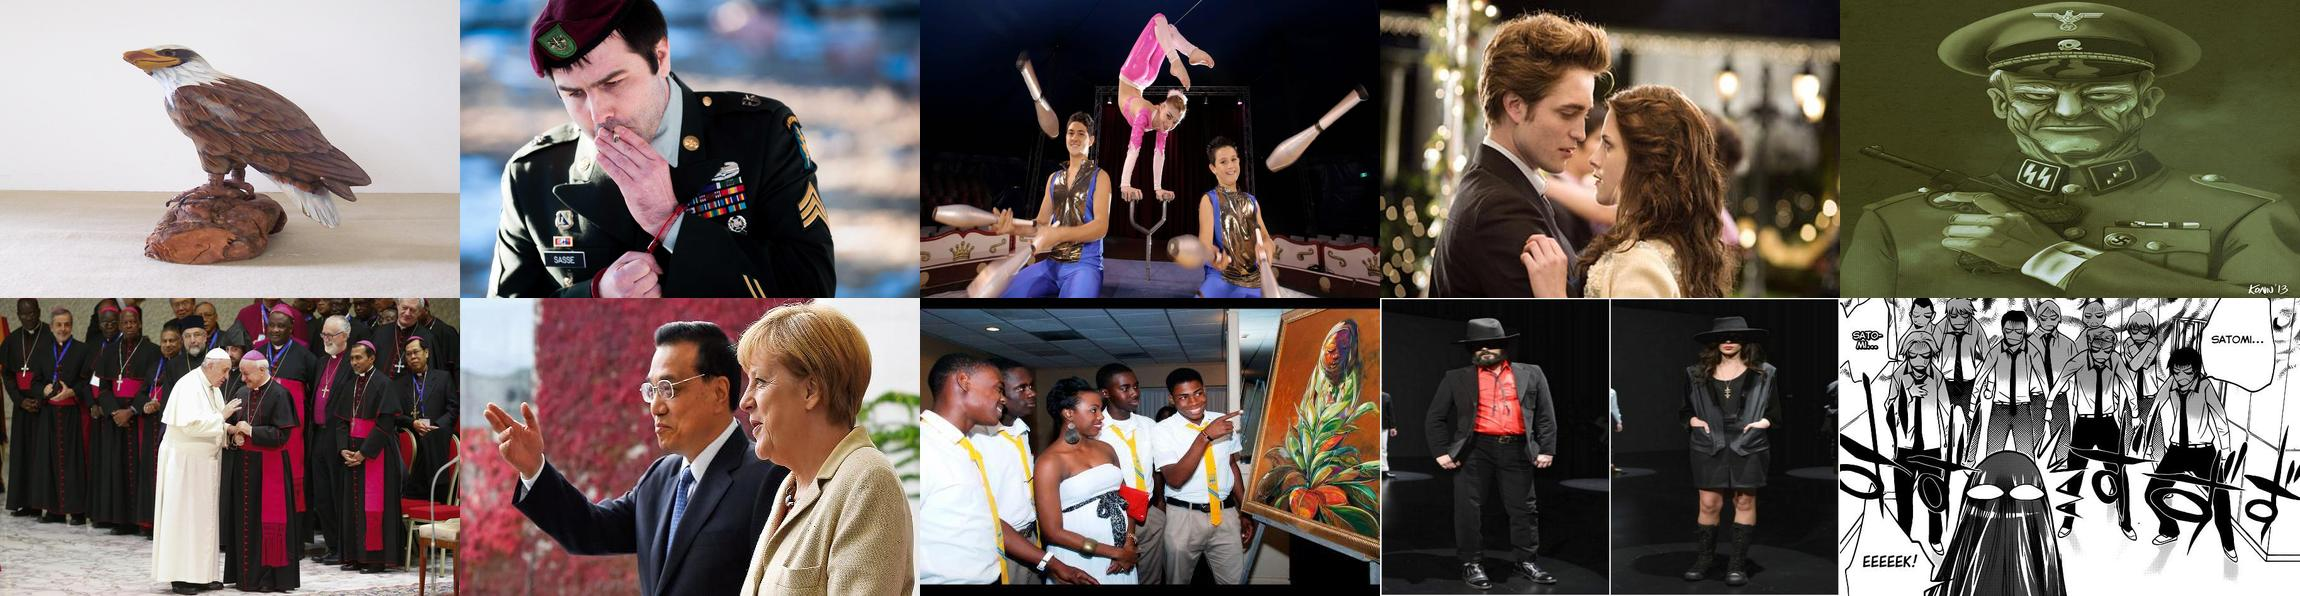
\includegraphics[scale=0.18]{fed_images/exp_w_sample.jpg}
    \caption{A random selection of images from the ExpW dataset}
    \label{figure:exp_w_sample}
\end{figure}

The ExpW dataset consists of 106,962 images, almost all (91,793) are annotated with the coordinates of the face present (some images contain multiple faces, however, only one face is annotated), and every annotated face shows one emotion out of happiness, neutral, sadness, surprise, fear, disgust, and anger. Images that are not annotated are not included in any of the following tests.

To determine the optimal combination of face detection and emotion detection algorithms for use in a resource-constrained robotic system, a comprehensive test was performed. This test involved pairing each face detection algorithm with each emotion detection algorithm to evaluate their performance. The primary goal was to find the best performing combination in terms of speed and accuracy for real-time applications on the robot. Each face detection and emotion detection instance was measured to calculate the average time taken for detection and prediction. Successful detections of faces and correct emotion predictions were meticulously recorded and compared to the actual emotions presented in the images of the data set.

\begin{table}[h!]
\centering
\caption{Average Detection Times in Milliseconds for Face and Emotion Detection Algorithms}
\begin{tabular}{|l|l|c|c|}
\hline
\textbf{Algorithm} & \textbf{Algorithm Name} & \textbf{Avg. Inf Time (ms)} & \textbf{Model Size (MB)}\\ \hline
\textbf{Face} & Tiny YOLO               & 25.0    &   22.4                                            \\ \cline{2-4} 
                        & Haar Cascade            & 40.7    &   1.19                    \\ \cline{2-4} 
                        & dlib                    & 45.6    &   0.696                   \\ \cline{2-4} 
                        & YOLO                    & 161.0   &   244                     \\ \hline
\textbf{Emotion} & MobileNetV2          & 13.6    &   69.8                                            \\ \cline{2-4} 
                        & ResNet50                & 95.3    &   187                      \\ \cline{2-4} 
                        & VGG16                   & 312.2   &   80.8                     \\ \hline
\end{tabular}
\label{tab:algorithm_detection_times_ms}
\end{table}


\begin{table}[h!]
\centering
\caption{Accuracy and Number of Face Detection for Model Combinations, out of a possible 91,793 faces}
\begin{tabular}{|l|c|c|}
\hline
\textbf{Model Combination}   & \textbf{Accuracy} & \textbf{No. of Face Detections} \\ \hline
dlib + MobileNetV2           & 37.06\%           & 56098                                   \\ \hline
dlib + ResNet50              & 37.77\%            & 56098                                   \\ \hline
dlib + VGG16                 & 34.52\%            & 56098                                   \\ \hline
Haar + MobileNetV2           & 46.63\%            & 76416                                   \\ \hline
Haar + ResNet50              & 47.81\%            & 76416                                   \\ \hline
Haar + VGG16                 & 44.52\%            & 76416                                   \\ \hline
Tiny YOLO + MobileNetV2      & 55.93\%            & 88332                                   \\ \hline
Tiny YOLO + ResNet50         & 57.36\%            & 88332                                   \\ \hline
Tiny YOLO + VGG16            & 51.94\%            & 88332                                   \\ \hline
YOLO + MobileNetV2           & 57.54\%            & 90773                                   \\ \hline
YOLO + ResNet50              & 59.02\%            & 90773                                   \\ \hline
YOLO + VGG16                 & 53.43\%            & 90773                                   \\ \hline
\end{tabular}
\label{tab:model_combinations_accuracy}
\end{table}

Since only one face in each image is annotated, all faces detectable in the image are compared to the one in the labels file, and the detected face that is closest (using Euclidian distance) to the listed face is considered the valid face for further analysis.

Tiny YOLO and YOLO, as face detection methods, provide the highest number of face detections, leading to improved overall accuracy when combined with emotion recognition models. Specifically, YOLO paired with ResNet50 achieves the highest accuracy in emotion recognition (59.02\%). Haar Cascade and dlib both achieved a lower number of face detections (resulting in lower overall accuracy) and a slower detection speed than Tiny YOLO which achieved a detection time of 0.0250 seconds on average. YOLO does provide a higher accuracy when it comes to the number of face detections and as a result, a higher overall accuracy; however, this increase in accuracy comes at the downside of 0.1610 seconds per face detection, more than 6 times slower than its Tiny counterpart for an overall accuracy increase of only 1.66\%. Thus, Tiny YOLO is the clear choice for facial recognition models. Among the emotion recognition models, ResNet50 generally outperforms MobileNetV2 and VGG16 across all face detection methods; however, considering the difference in detection times for ResNet50 (95.3 milliseconds) and MobileNetV2 (13.6 milliseconds) the choice is not as obvious and both could be left as suitable options depending on the need for higher accuracy or higher detection speed. Another consideration in a resource-constrained environment is the size of the models. ResNet50 has the largest model size at 187MB leaving less memory for the robots other processes to work with. This leaves the best combination for overall accuracy, memory efficiency, and speed to be Tiny YOLO + MobileNetV2 with it only requiring 92.2 MB of memory for both models.

Finally, the performance of the model is evaluated directly on a robot. The system is designed to be standalone and operate without relying on a connected PC, so testing the models in this context is essential.

\begin{table}[h!]
\centering
\caption{Average Detection Times in Milliseconds for Face and Emotion Detection Algorithms performed on the TurtleBot4}
\begin{tabular}{|l|l|c|}
\hline
\textbf{Algorithm Type} & \textbf{Algorithm Name} & \textbf{Average Detection Time (ms)} \\ \hline
\textbf{Face Detection} & Tiny YOLO               & 697.4                                \\ \cline{2-3} 
                        & Haar Cascade            & 491.7                                \\ \cline{2-3} 
                        & dlib                    & 216.2                                \\ \cline{2-3} 
                        & YOLO                    & 6846.5                               \\ \hline
\textbf{Emotion Detection} & MobileNetV2          & 124.7                                \\ \cline{2-3} 
                        & ResNet50                & 1334.3                               \\ \cline{2-3} 
                        & VGG16                   & 5384.2                               \\ \hline
\end{tabular}
\label{tab:algorithm_detection_times_ms_robot}
\end{table}

The results of the Turtlebot4 tests are summarised in the table above. It should be noted that the performance of face detection methods exhibits a significant reversal when implemented on a robot with limited resources. Surprisingly, Tiny YOLO, which was initially the fastest, was surpassed by both dlib and Haar Cascade. Even Haar Cascade, was outperformed by dlib by a considerable margin. This behaviour could be due to a couple things, the Turtlebot 4 does not possess any GPUs unlike the training PC and it is possible that YOLO is using GPU acceleration to improve detection times. The other possibility is that YOLO leverages the vastly increased number of CPU cores on the training PC to perform parallel computations more efficiently, distributing the workload across multiple cores. However, when deployed on the Turtlebot4, which has significantly fewer cores, YOLO's speed advantage diminishes, leading to slower inference times compared to simpler models like dlib and Haar Cascade.

The results for the emotion models remained consistent with the original tests conducted on the training PC. Among these models, MobileNetV2 stands out as the fastest and most accurate choice for direct implementation on a robot. However, the selection of a face detection model is more nuanced. For maximum accuracy, Tiny YOLO is the preferred option, closely trailing full YOLO in accuracy, but with each detection taking less than a second as opposed to 6.8 seconds. If rapid detections are a priority, dlib is a clear choice, while Haar Cascade provides a balanced compromise between accuracy and inference speed.